\chapter{Riconoscimento degli Oggetti}
\label{cap:riconoscimento}
\thispagestyle{empty}

\begin{quotation}
{\footnotesize
\noindent\emph{Marty: Ok, rilassati Doc, sono io, sono io Marty! \\
Doc: No, non può essere \dots io ti ho rimandato nel futuro! \\
Marty: Lo so mi hai rimandato indietro nel futuro, ma sono tornato, sono tornato dal futuro! \\
Doc: Grande Giove!}
\begin{flushright}
Ritorno al Futuro, parte II
\end{flushright}
}
\end{quotation}
\vspace{0.5cm}

\section{Introduzione}

In questo capitolo descriveremo il riconoscimento di oggetti. Il riconoscimento degli oggetti si basa sull'estrazione di features geometriche e la loro classificazione tramite un classificatore fuzzy ad albero, che sfrutta il reasoner descritto nel \autoref{cap:reasoning}.
Il sistema qui descritto si pone l'obbiettivo di dimostrare una possibile applicazione del sistema di classificazione basato sulla conoscenza di un esperto, delineando le metodologie per estrarre feature e classificarle. Tuttavia un sistema completo di classificazione delle feature completo può estrarre molta più informazione dall'immagine, sia come quantità di feature estraibili (ad esempio estraendo coniche e piani), sia come informazioni caratterizzanti (ad esempio aggiungendo il colore).

Il sistema implementato è pensato principalmente per estrarre quadrilateri e cluster, e analizzarli. Questa scelta è stata fatta perchè la maggior parte degli oggetti presenti in un ambiente, come una stanza o un ufficio, si compone di oggetti planari rettangolari (porte, finestre, armadi). Questi oggetti spesso sono caratterizati da componenti più piccole, come ad esempio le maniglie, che hanno la caratteristica di avere una geometria complessa. Questo causa una massicia concentrazione di keypoint, rendendo possibile la loro individuazione tramite algoritmi di clustering.

Il riconoscimento avviene su più livelli: prima vengono analizzate le feature più facili da riconoscere. In seguito per ogni feature riconosciuta viene effettuatta una analisi ad alto livello.

\section{Individuazione delle features geometriche}

Le feature geometriche sono individuate da algoritmi specifici. Tuttavia è stata definita una struttura di base, rappresentata dalla classe feature. La classe feature implementa l'interfaccia tra il classificatore e l'algoritmo di riconoscimento nell'immagine.
La \autoref{fig:feature} mostra la struttura delle classi del sistema implementato. Come si nota, la classe feature implementa due strutture dati:

\begin{description}
 \item [FeatureMap] è un dizionario che contiene i dettagli dell'oggetto riconosciuto, con il nome delle feature e il loro valore.
 \item [ClassificationMap] è un dizionario che contiene tutte le classificazioni attribuite all'oggetto, con il relativo grado di apparteneza.
\end{description}

La FeatureMap è popolata tramite il metodo setFeature a partire dai dati caratteristici della stessa.
La ClassificationMap è popolata tramite il metodo addClassification. La classe feature contiene ulteriori metodi per l'analisi semantica dell'oggetto.

\begin{figure}[ht]
  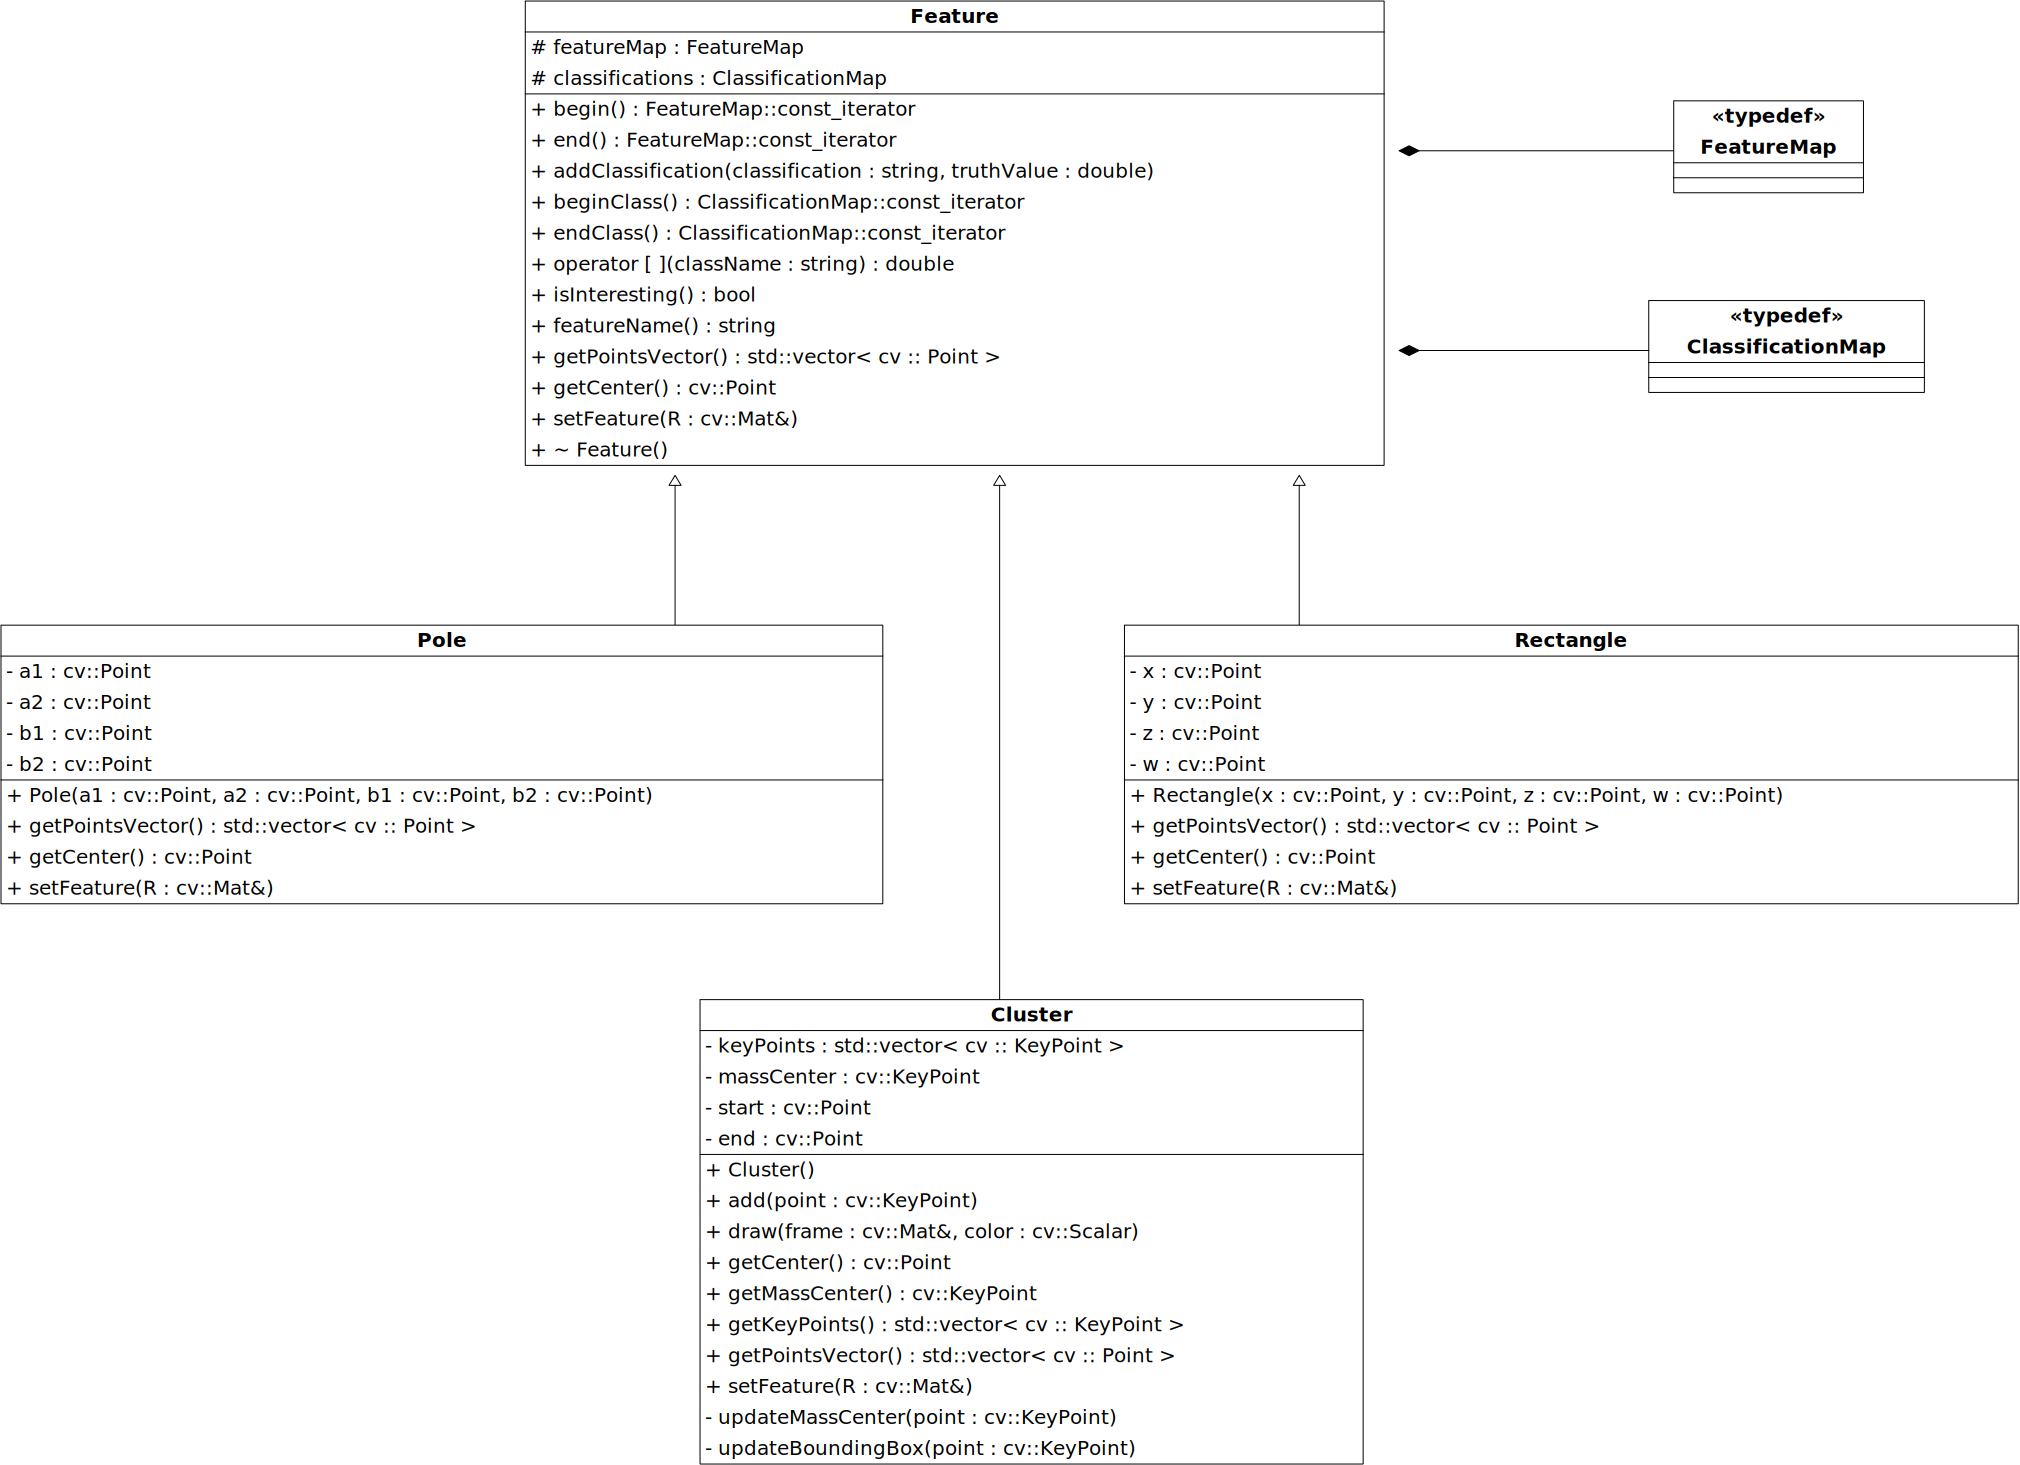
\includegraphics[width=\textwidth]{diagrammi/Feature}
  \caption{Classe Feature e sottoclassi implementate}
  \label{fig:feature}
\end{figure}

Di seguito vengono discussi gli algoritmi implementati per il riconoscimento delle feature geometriche.
La base di partenza per tutti gli algoritmi considerati è l'immagine rettificata della telecamera, ossia l'immagine senza la distorsione causata dalle caratteristiche costruttive della lente, ovvero la distorsione radiale e tangenziale.

\subsection{Quadrilateri}

L'algoritmo di riconoscimento di quadrilateri si basa principalmente sull'algortimo di Canny~\cite{4767851} per il riconoscimento dei bordi e sulla trasformata di Hough probabilistica~\cite{matas2000robust} per estrarre le linee, o più precisamente, i segmenti, dalla mappa dei bordi.

Le linee estratte contengono, quando l'ambiente è minimamente complesso, molte linee spurie. Inoltre, i quadrilateri interessanti sono composti da due linee approssimativamente orizzontali e due linee approssimativamente verticali. Per questo è stato implementato un algoritmo di filtraggio delle linee in grado di dividere le linee orizzontali da quelle verticali e dal rumore. Per discriminare le linee si utilizzano i dati dell'odometria del robot. Conoscendo infatti la posa del robot approssimativamente, data l'odometria, è possibile stimare l'inclinazione dell'orizzonte e della linea perpendicolare ad esso. Le linee orizzontali e verticali sono quelle la cui inclinazione, espressa in angolo rispetto all'asse delle ascisse, non supera una determinata soglia rispetto, rispettivamente, all'orizzonte e alla sua perpendicolare.

Una volta riconosciute le linee verticali e orizzontali viene applicato l'\autorefA{alg:quad-det} per riconoscere quadrilateri e pali.
Viene considerato palo una coppia di linee con un fattore di forma estremamente schiacciato verticalmente. Nell'algoritmo descritto V rappresenta il vettore di linee verticali (ordinate da destra a sinistra), H l'insieme delle linee orizzontali, Q l'insieme di quadrilateri trovati.

\begin{algorithm}[ht]
\caption{QuadrilateralDetector}
\begin{algorithmic}[1] 
\label{alg:quad-det}
\FOR{$i \in \lbrace 0, VerticalLinesNumber -1 \rbrace$}
  \STATE $v_{1} \leftarrow V[i]$
  \STATE $v_{2} \leftarrow V[i+1]$
  \IF{$v_{1}$ and $v_{2}$ are not poles}
    \FORALL{$(h_{1},h_{2}) \in H \times H$}
      \STATE $x \leftarrow$ findInterception($h_{1}$, $v_{1}$);
      \STATE $y \leftarrow$ findInterception($h_{1}$, $v_{2}$);
      \STATE $z \leftarrow$ findInterception($h_{2}$, $v_{2}$);
      \STATE $w \leftarrow$ findInterception($h_{2}$, $v_{1}$);
      \IF{$x,y,z,w$ are the vertices of a quadrilateral $q$}
	\STATE $Q = Q \cup \lbrace q \rbrace$
      \ENDIF
    \ENDFOR
  \ENDIF
\ENDFOR
\RETURN Q
\end{algorithmic}
\end{algorithm}

Questo algoritmo si basa su una considerazione fondamentale per ridurre la complessità del calcolo, ossia che è altamente probabile che un rettangolo interessante si trovi tra due linee verticali consecutive. Questa considerazione è sostenuta dal fattore di forma dell'immagine, che è largo, e dal fattore di forma della maggior parte dei quadrilateri interessanti, che solitamente sono più stretti che larghi. Questa considerazione non si può tuttavia estendere al caso delle linee orizzontali, per le motivazioni opposte, e per questo è fatta in maniera esaustiva.


Per discriminare se un insieme di punti formano o meno un quadrilatero vengono utilizzati due euristiche, a seconda del riconoscimento effettuato.
L'euristica più semplice consiste nel considerare tutto ciò che non è un palo come un quadrilatero. Questa euristica in generale è pessima, ma funziona molto bene, avendo un tasso di recupero decisamente alto, quando il riconoscimento è localizzato.

L'altra euristica possibile che abbiamo sviluppato consiste nello sfruttare le proprietà delle combinazioni convesse. Una combinazione convessa è definita come una combinazione lineare con coefficenti positivi e la cui somma vale 1. L'insieme delle combinazioni convesse di un insieme di punti generano l'involucro convesso dell'insieme.
Nel nostro caso, preso un segmento riconosciuto come possibile lato del quadrilatero, possiamo calcolare qualsiasi punto al suo interno tramite la formula:

\begin{equation}
  x = \alpha\cdot a + (1 - \alpha)\cdot b = b + \alpha\cdot(a - b)
\end{equation}

Dove $a$ e $b$ sono gli estremi del segmento e $x$ è un punto al suo interno, i coefficenti di combinazione convessa sono $\alpha$ e $1 - \alpha$.
Come si nota dalla formula $\alpha = 0$ se $x \equiv b$ e $\alpha = 1$ se $x \equiv a$.
Idealmente, per i vertici di un quadrato, si avrà $\alpha=1$ o $\alpha=0$ se si calcola il coefficente del vertice rispetto ai due segmenti adiacenti.

Se si prova a calcolare il valore di $\alpha$ con la stessa formula per un punto fuori dal segmento si ottiene un valore maggiore di uno o minore di zero.

L'euristica proposta si basa sulle considerazioni fatte sopra, supponendo che a causa del rumore e altri fattori, i vertici del quadrato riconosciuto si possano trovare all'interno o all'esterno del segmento. Viene quindi calcolato il valore di combinazione convessa di ciascun vertice e, fissata una soglia, viene riconosciuto come quadrato solo un insieme di segmenti i cui vertici hanno $\alpha=1$ o $\alpha=0$, a meno della soglia.

\subsection{Cluster}

I cluster vengono riconosciuti estraendo i keypoint dall'immagine tramite l'algortimo FAST~\cite{rosten_2006_machine}.

Una volta estratti i keypoint, vengono estratti i cluster interessanti tramite l'algoritmo DBSCAN~\cite{ester1996density}.
DBSCAN è un algoritmo che si basa sulla distanza tra i punti. Due punti vengono considerati vicini se la distanza tra di loro è minore di una determinata soglia. Vengono quindi inseriti in un unico cluster tutti i punti che sono raggiungibili tramite la relazione di vicinanza. Ciò significa che tutti i vicini di un punto sono inseriti nello stesso cluster, e allo stesso modo i vicini dei vicini, ricorsivamente.
I cluster che non hanno abbastanza punti al loro interno vengono scartati e considerati come rumore.

\section{Integrazione con il reasoning}
Una volta riconosciute le feature interessanti, vengono calcolati i descrittori di tali feature. I descrittori delle feature vengono inseriti nella FeatureMap, per poter comunicare la feature riconosciuta al classificatore fuzzy.
Viene effettuata la rotazione delle coordinate in modo da avere i quadrilateri riconosciuti il più possibile orientati verticalmente. Questo facilita il compito del reasoner, in quanto attualmente l'operatore ``on'' supporta solo intervalli semplici e non aree o intervalli generici (si veda \autoref{cap:reasoning}).
Le richieste di classificazione vengono, per quanto possibile, inviate contemporaneamente al reasoner, in modo da rendere possibile l'analisi delle relazioni tra gli oggetti riconosciuti. Viene poi popolata, con i dati provenienti dal reasoner, la ClassificationMap. Questo è reso possibile perchè ogni feature inviata è associata a un indice univoco.


\section{Livelli di riconoscimento}



